\documentclass{article}
\usepackage[T1]{fontenc}

\def \figwidth{0.8\textwidth}

%% The packages beton, concmath, and ccfonts are LaTeX packages that
%% change the default text fonts from Computer Modern to
%% Concrete. Packages beton and ccfonts also slightly increase the
%% default value of \baselineskip to account for the rather heavier
%% weight of the Concrete fonts.
\usepackage{beton}
\usepackage{concmath}
\usepackage{ccfonts}
\usepackage{eulervm}

\usepackage{graphicx}
\usepackage{listings}
\usepackage{float}
\usepackage[margin=2.5cm]{geometry}
\usepackage{verbatim}
\usepackage{subfigure}
\usepackage{wrapfig}

\def \insertt {{\tt vtkDataArray::InsertNextTuple~}}
\def \copydata {{\tt vtkDataSetAttributes::CopyData~}}

\begin{document}
\date{}
\title{Tuning VTK data arrays}
\maketitle
As data structures get more laden with features, performance tends to
degrade over times. Bread-and-butter data containers in VTK suffer
from this as well. On the bright side, we find that simple
optimization doubles the speed of two common operations, \insertt and
\copydata, with no sacrifice to usability. As a result, the speed of
{\tt vtkSynchronizedTemplates3D} is improved by 6 percent.

We hope that this experience serves as motivation to extent this
effort to other common VTK data container operations. We believe that
such efforts will lead to significant across-the-board performance
improvement.

\section{How slow are we, really?}
To get a sense of how fast VTK is and how fast it ``should'' be. We
compare it with STL and memcpy. STL makes a more relevant comparison
here, while memcpy gives us a sort of time unit. From the results
below, one can perhaps say that while VTK is slow, it is not
embarrassingly slow.

\begin{table}[h]
\centering
\begin{tabular}{r|c|c|c}
 &  VTK & STL & memcpy\\
\hline
\insertt & 0.21 & 0.16 & 0.02 \\
\hline
\copydata & 0.52 &  0.13 &  0.06\\
\end{tabular}
\caption{Time (in seconds) of inserting 1M points 10 times and
  averaged over 10 runs. The compilation is in CMAKE RelWithDebInfo mode.}\
\label{tab:initial}
\end{table}

\subsubsection*{Code References}
\begin{itemize}
\item Run {\tt ./arraytest -op insert} to get the VTK insertion time.
\item Run {\tt ./arraytest -op insert -c} to get the memcpy insertion time.
\item Run {\tt ./arraytest -op insert -stl} to get the stl insertion time.
\end{itemize}

\section{Speeding up \insertt}

\begin{figure}[H]
\centering{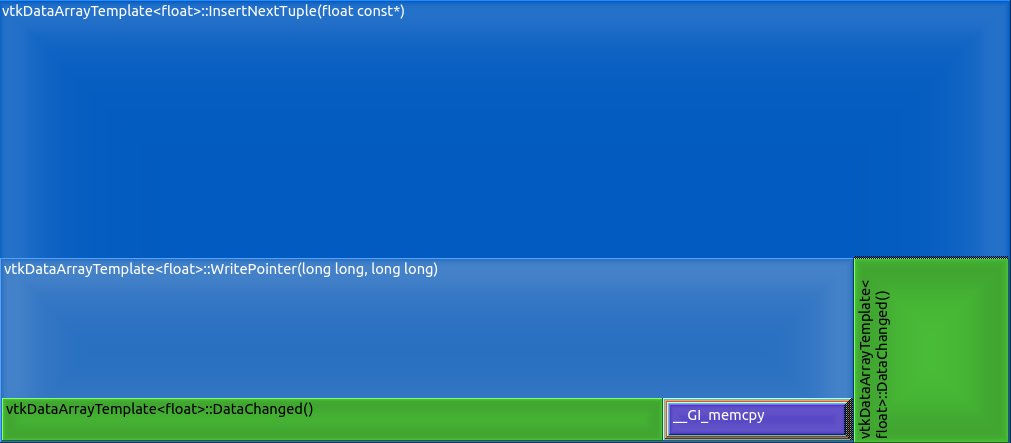
\includegraphics[width=0.5\textwidth]{insertnexttuple.png}}
\caption{Profiling of \insertt using callgrind and visualized in kcachegrind}
\label{fig:insert}
\end{figure}

The profiling shows that the bottle-neck is WritePointer() and
in the body of InsertNextTuple().

To attack the first bottleneck, we introduce a protected method
AppendPointer() that takes advantage of the fact that the caller is
already calling DataChanged(), so its own DataChanged() can be
skipped.  We can also remove some extra variables and a conditional
because we know we are inserting to the tail.

The slowest statement in the second bottle neck turns out to be a
division that computes the next id from the total length and the
number of components. This takes up more than half of the time! We
remove this division by introducing an extra counter variable and
incrementing it instead.

The optimization more than doubles the speed. We are now beating the
STL implementation.
\begin{table}[h]
\centering
\begin{tabular}{r|c|c|c}
         &  VTK (before) & VTK (after) & Speed-up
\\
\hline
\insertt & 0.21          & 0.1         & $\times$2.1
\\
\end{tabular}
\caption{Speed up of the test referenced in Table~\ref{tab:initial}}
\end{table}


\subsubsection*{Code References}
\begin{itemize}
\item Run {\tt ./arraytest --op insert}.
\end{itemize}

\section{Speeding up \copydata}

\begin{figure}[H]
\centering{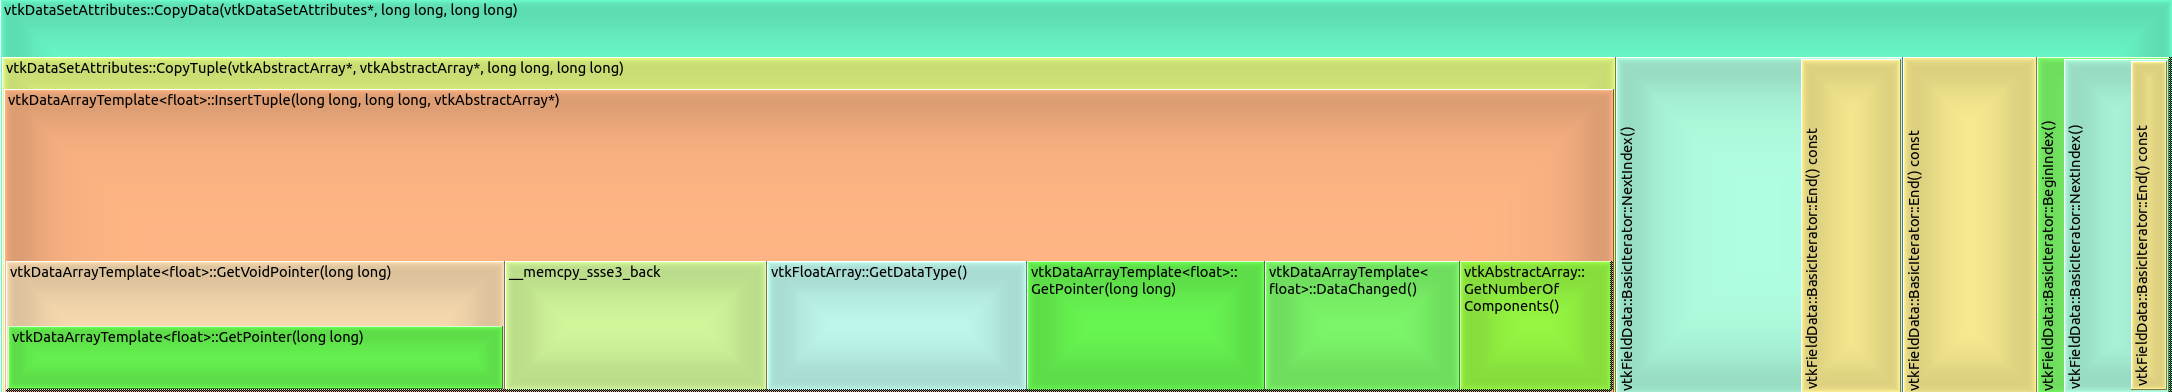
\includegraphics[width=\textwidth]{copydata.png}}
\caption{Profiling of \copydata using callgrind and visualized in kcachegrind}
\label{fig:insert}
\end{figure}

The profiling shows a lot of calls to GetNumberOfComponents() and
GetDataTypes() calls, all coming from safety checks done in
InsertTuple().  We know these are completely unnecessary if the copy
source does not change. So our solution is to create a CopyHelper
class that is instantiated with the source and destination and
provides a copy method that just has the source and destination index,
but not the source object pointer.  Since the source does not change,
we can safely call a trimmed protected method InsertTupleFast() that
does not do those safety checks. Inside CopyHelper, we also use
simple array data structures to support traversal of the various
fields, which are faster than using vtkFieldData::BasicIterator.

Using CopyHelper on the caller side amounts to adding one call to
construct CopyHelper, and replace {\tt destination->CopyData(i,j,source)}
by {\tt copyHelper->Copy(i,j)}.


The optimization yields a 50 percent speed-up.
\begin{table}[h]
\centering
\begin{tabular}{r|c|l}
\copydata & CopyHelper & Speed-up
\\\hline
 0.52          & 0.34         & $\times$1.52
\\
\end{tabular}
\caption{Speed up of the test referenced in Table~\ref{tab:initial}}
\end{table}


\subsubsection*{Code References}
\begin{itemize}
\item For using the existing vtkDataSetAttributes::CopyData, run {\tt ./arraytest --op copy}.
\item For using the copy helper, run {\tt ./arraytest -op copy -helper}.
\end{itemize}

\subsection{``Lazy'' Copy: A Coherence-Sensitive Copier}

We also investigated using ``lazy copy'' to replace copying ranges of
data by memcpy, since memcpy() is so fast.  When a caller calls {\tt
  LazyCopy::Copy(i,j)}, instead of actually performing the copying, it
tries to accumulate a contiguous range and perform copying only when
the continuous range ends---or when the caller explicitly calls {\tt
  LazyCopy::Flush}.

Unlike the previous optimization techniques, lazy copying loses some
functionality: During the copying process, the caller cannot read
destination data since copying might not have occurred; the caller also
must remember to ``flush'' in the end.

The actual speed-up gained also varies depending on whether these
continuous ranges occur in the input. Nonetheless, in the best case
---as in our simple test, we gain an order of magnitude speed-up by performing
exactly one memcpy:
\begin{table}[h]
\centering
\begin{tabular}{r|c|l}
\copydata & LazyCopy & *Speed-up
\\\hline
 0.52          & 0.05         & $\times$10
\\
\end{tabular}
\caption{Speed up of the test referenced in
  Table~\ref{tab:initial}. We mark Speed-up with * because the result
  represents the best achievable.}
\end{table}

\subsubsection*{Code References}
\begin{itemize}
\item Run {\tt ./arraytest -op copy -lazy}.
\end{itemize}

\section{Impact on filters}
We compare the speed of vtkSynchronizedTemplates before and after the
speed improvement. The performance gain is small but noticeable:
\begin{table}[h]
\centering
\begin{tabular}{r|c|l}
\copydata & CopyHelper(speed-up) & LazyCopy(speed-up)
\\\hline
 1.32        & 1.24($\times$1.06)    & 1.26($\times$1.04)
\\
\end{tabular}
\caption{Speed up of vtkSynchronizedTemplates.}
\end{table}

The relatively small percentage gain is because, for this particular
filter, the time spent on inserting points and copying is a fairly
small percentage of the overall time. We suspect that optimizing
other data container routines such as vtkCellArray will give us
further speed-up.

We also note that lazy copy does not help here, this is because the
average range length is only about 2, so the saving is not enough to
overcome the overhead.
%% 1.26


\section{Discussion}


We need to have performance benchmark tests.  There is no hard
success/failure, but somehow we need to be able to keep track of the
performance in various configurations. The performance score can be in
terms of standard c libraries.



\end{document}

original,

leo:tbb-build$ ./arraytest --stl
Time: 0.152054 seconds
leo:tbb-build$ ./arraytest
Time: 0.201302 seconds

#use AppendPointer() for InsertNextTuple(float* )
# so, some DataChanged calls are skipped
leo:tbb-build$ ./arraytest
Time: 0.184821 seconds

#skipping all DataChanged calls
leo:tbb-build$ ./arraytest
Time: 0.174877 seconds

# not computing the division:
leo:tbb-build$ ./arraytest
Time: 0.080606 seconds

some surprise:

- change for (.. i<3; i++) -> memcpy( , 3*sizeof(.))
is slower in release mode
- preallocate is slower


Using CopyHelper is about 2 times faster





# original time for contouring
leo:tbb-build$ ./pcontour --extent 200
0 threads
64 pieces
Report output
time: 1.32152 seconds
1359481 points, 2711872 cells 2711872 cell data values


#  (with improved InsertNextTuple())
leo:tbb-build$ ./pcontour --extent 200
0 threads
64 pieces
Report output
time: 1.34502 seconds
1359481 points, 2711872 cells 2711872 cell data values

leo:tbb-build$ ./pcontour --filter thresh --extent 100
0 threads
64 pieces
Report output
time: 3.76379 seconds
8120601 points, 8000000 cells 8000000 cell data values

./pcontour --extent 100 --filter surf
0 threads
64 pieces
Report output
time: 35.121 seconds
240002 points, 240000 cells

# with lazy copy

leo:tbb-build$ ./pcontour --extent 200
0 threads
64 pieces
Report output
time: 1.29274 seconds
1359481 points, 2711872 cells 2711872 cell data values

leo:tbb-build$ ./pcontour --filter thresh --extent 100
0 threads
64 pieces
Report output
time: 3.31758 seconds
8120601 points, 8000000 cells 8000000 cell data values



1.216704

